\section{Analisi}
\subsection{Casi d'uso}
I casi d'uso rappresentano uno strumento fondamentale nell'analisi dei requisiti di un sistema \textit{software}. Essi descrivono 
le interazioni tra gli utenti (o altri sistemi esterni) e il sistema in esame, illustrando come questo debba comportarsi per 
soddisfare le esigenze degli \textit{stakeholder}.\\
Ogni caso d'uso riporta:
\begin{itemize}
    \item \textbf{Attore}: attori coinvolti nel caso d'uso;
    \item \textbf{Descrizione}: descrizione del caso d'uso;
    \item \textbf{Pre-condizione}: condizioni vere prima del verificarsi del caso d'uso;
    \item \textbf{Post-condizione}: condizioni vere dopo il verificarsi del caso d'uso;
    \item \textbf{Scenario}: sequenza specifica di eventi che si verifica quando un attore interagisce con il sistema 
                             per raggiungere un obiettivo;
\end{itemize}
Nelle sezioni seguenti, esamineremo in dettaglio i casi d'uso, che ho identificato durante lo studio del capitolato del progetto.

\subsubsection{UC 1 - \textit{Login}}
\begin{figure}[H]
    \vspace{2em}
    \centering
    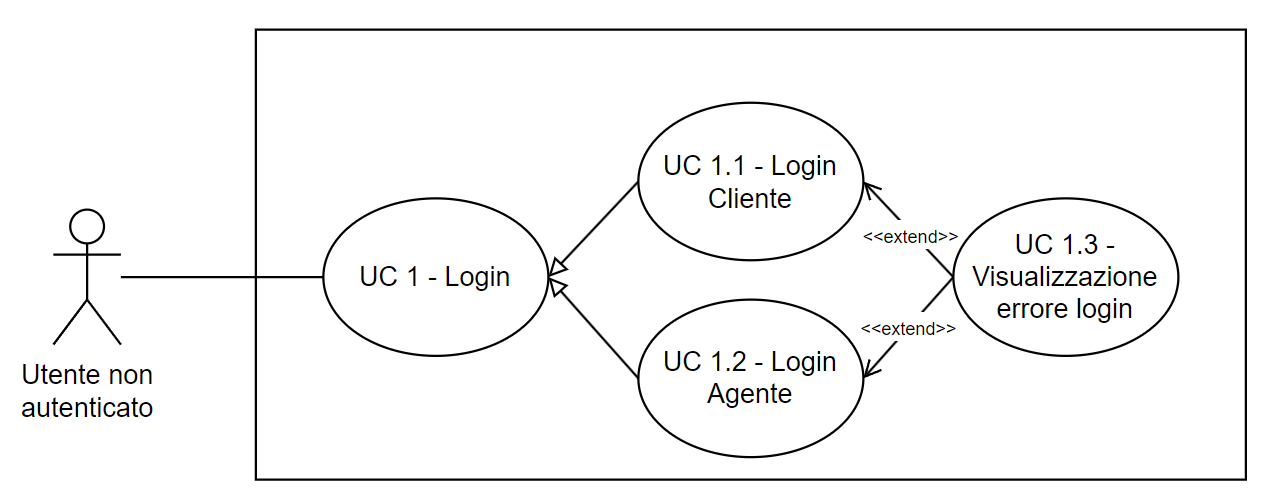
\includegraphics[width=0.75\columnwidth]{img/usecase/UC 1.png}
    \caption{\textit{Use Case} 1: \textit{Login} Utente}
    \label{fig:uc_1}
\end{figure}

\begin{usecase}{ 1}{\textit{Login} utente}
    \usecaseactors{Utente non autenticato.}
    \usecasedesc{L'utente ha inserito \textit{username} e \textit{password} per autenticarsi nell'\textit{app}.}
    \usecasepre{L'utente ha avviato l'\textit{app}.}
    \usecasepost{L'utente è autenticato nel sistema o ha ricevuto un errore.}
    \usecasescen{
        \begin{itemize}
            \item L'utente visualizza la schermata di \textit{login} di {\movi};
            \item L'utente inserisce lo \textit{username};
            \item L'utente inserisce la \textit{password};
            \item L'utente preme il pulsante per effettuare il \textit{login};
            \item L'utente viene autenticato ed entra nell'applicazione.
        \end{itemize}}
    \label{uc:uc_1}
\end{usecase}

\begin{usecase}{ 1.1}{\textit{Login} cliente}
    \usecaseactors{Utente non autenticato.}
    \usecasedesc{L'utente è un cliente dell'azienda e vuole autenticarsi nell'\textit{app}.}
    \usecasepre{L'utente ha avviato l'\textit{app}.}
    \usecasepost{L'utente è autenticato come cliente nel sistema o ha ricevuto un errore. Viene portato 
                 nella \textit{homepage} e nulla cambia rispetto la vecchia versione dell'\textit{app}.}
    \usecasescen{
        \begin{itemize}
            \item L'utente visualizza la schermata di \textit{login} di {\movi};
            \item L'utente inserisce lo \textit{username};
            \item L'utente inserisce la \textit{password};
            \item L'utente preme il pulsante per effettuare il \textit{login};
            \item L'utente viene autenticato e visualizza la \textit{homepage} dell'applicazione.
        \end{itemize}}
    \label{uc:uc_1.1}
\end{usecase}

\begin{usecase}{ 1.2}{\textit{Login} agente}
    \usecaseactors{Utente non autenticato.}
    \usecasedesc{L'utente è un agente dell'azienda e vuole autenticarsi nell'\textit{app}.}
    \usecasepre{L'utente ha avviato l'\textit{app}.}
    \usecasepost{L'utente è autenticato come agente nel sistema o ha ricevuto un errore. Viene portato 
                 nella \textit{homepage} agenti.}
    \usecasescen{
        \begin{itemize}
            \item L'utente visualizza la schermata di \textit{login} di {\movi};
            \item L'utente inserisce lo \textit{username};
            \item L'utente inserisce la \textit{password};
            \item L'utente preme il pulsante per effettuare il \textit{login};
            \item L'utente viene autenticato e visualizza la \textit{homepage} agenti dell'applicazione.
        \end{itemize}}
    \label{uc:uc_1.2}
\end{usecase}

\begin{usecase}{ 1.3}{Visualizzazione errore \textit{login}}
    \usecaseactors{Utente non autenticato.}
    \usecasedesc{L'utente vuole autenticarsi nell'\textit{app} ma ha inserito \textit{username} o \textit{password} non validi.}
    \usecasepre{L'utente ha avviato l'operazione di \textit{login}.}
    \usecasepost{L'utente visualizza un messaggio che lo avvisa del fallimento dell'operazione di \textit{login}.}
    \usecasescen{
        \begin{itemize}
            \item L'utente visualizza la schermata di \textit{login} di {\movi};
            \item L'utente inserisce lo \textit{username};
            \item L'utente inserisce la \textit{password};
            \item L'utente preme il pulsante per effettuare il \textit{login};
            \item L'utente visualizza un errore.
        \end{itemize}}
    \label{uc:uc_1.3}
\end{usecase}

\subsubsection{UC 2 - Operazioni disponibili nella \textit{homepage} agenti}
\begin{figure}[H]
    \vspace{2em}
    \centering
    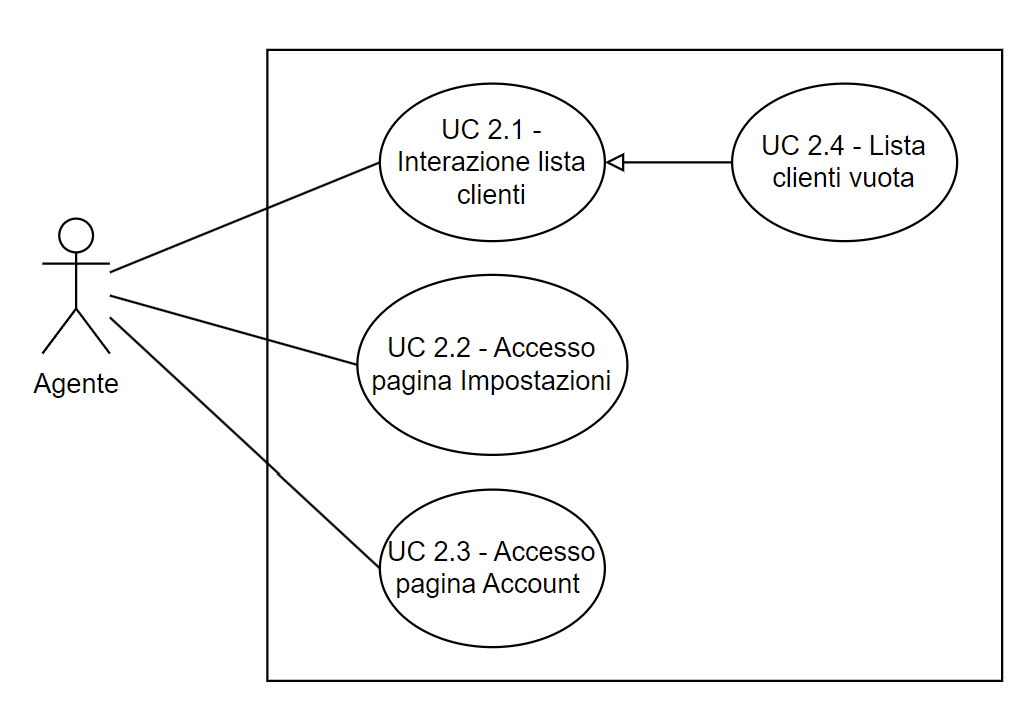
\includegraphics[width=0.75\columnwidth]{img/usecase/UC 2.png}
    \caption{\textit{Use Case} 2: Operazioni disponibili nella \textit{homepage} agenti}
    \label{fig:uc_2}
\end{figure}

\begin{usecase}{ 2.2}{Accesso pagina Impostazioni}
    \usecaseactors{Agente.}
    \usecasedesc{L'agente, cliccando nell'apposito menu il pulsante "Impostazioni", viene spostato nella pagina Impostazioni.}
    \usecasepre{L'utente si è autenticato con successo ed e stato riconosciuto come agente, quindi visualizza la 
                \textit{homepage} agenti.}
    \usecasepost{L'agenti viene spostato nella nella pagina Impostazioni.}
    \usecasescen{
        \begin{itemize}
            \item L'agente visualizza la \textit{homepage} agenti;
            \item L'agente visualizza il menu;
            \item L'agente clicca il pulsante "Impostazioni";
            \item L'agente viene spostato nella pagina Impostazioni.
        \end{itemize}}
    \label{uc:uc_2.2}
\end{usecase}

\begin{usecase}{ 2.3}{Accesso pagina Account}
    \usecaseactors{Agente.}
    \usecasedesc{L'agente, cliccando nell'apposito menu il pulsante "Account", viene spostato nella pagina Account.}
    \usecasepre{L'utente si è autenticato con successo ed e stato riconosciuto come agente, quindi visualizza la 
                \textit{homepage} agenti.}
    \usecasepost{L'agenti viene spostato nella nella pagina Account.}
    \usecasescen{
        \begin{itemize}
            \item L'agente visualizza la \textit{homepage} agenti;
            \item L'agente visualizza il menu;
            \item L'agente clicca il pulsante "Account";
            \item L'agente si sposta nella pagina "Account"
        \end{itemize}}
    \label{uc:uc_2.3}
\end{usecase}

\begin{usecase}{ 2.4}{Lista clienti vuota}
    \usecaseactors{Agente.}
    \usecasedesc{L'agente che ha una lista clienti vuota visualizza il messaggio 
                 "nessun cliente trovato".}
    \usecasepre{
        \begin{itemize}
            \item L'utente si è autenticato con successo ed e stato riconosciuto come agente, quindi visualizza la 
                \textit{homepage} agenti;
            \item La lista clienti è vuota.
        \end{itemize}}
    \usecasepost{L'agente visualizza il messaggio "nessun cliente trovato".}
    \usecasescen{
        \begin{itemize}
            \item L'agente visualizza la \textit{homepage} agenti;
            \item L'agente ha la lista clienti vuota;
            \item L'agente visualizza il messaggio "nessun cliente trovato" al posto della lista.
        \end{itemize}}
    \label{uc:uc_2.4}
\end{usecase}

\subsubsection{UC 2.1 - Interazioni con la lista clienti}
\begin{figure}[H]
    \vspace{2em}
    \centering
    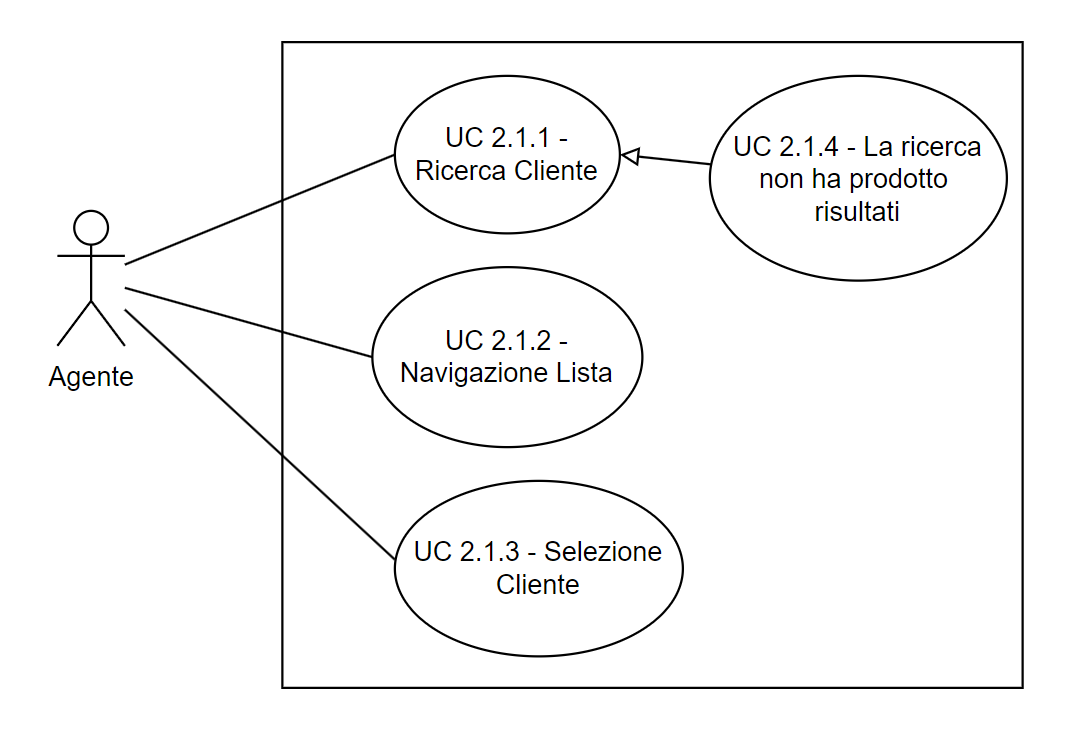
\includegraphics[width=0.75\columnwidth]{img/usecase/UC 2.1.png}
    \caption{\textit{Use Case} 2.1: Interazioni con la lista clienti}
    \label{fig:uc_2.1}
\end{figure}

\begin{usecase}{ 2.1.1}{Ricerca cliente}
    \usecaseactors{Agente.}
    \usecasedesc{L'agente ricerca un cliente specifico all'interno della lista clienti.}
    \usecasepre{
        \begin{itemize}
            \item L'utente si è autenticato con successo ed è stato riconosciuto come agente, quindi visualizza la 
                \textit{homepage} agenti;
            \item La lista clienti non è vuota.
    \end{itemize}}
    \usecasepost{L'agente visualizza il cliente ricercato.}
    \usecasescen{
        \begin{itemize}
            \item L'agente visualizza la \textit{homepage} agenti;
            \item L'agente visualizza la lista clienti;
            \item L'agente ricerca un cliente nella lista clienti;
            \item L'agente visualizza il cliente ricercato.
        \end{itemize}}
    \label{uc:uc_2.1.1}
\end{usecase}

\begin{usecase}{ 2.1.2}{Navigazione lista}
    \usecaseactors{Agente.}
    \usecasedesc{L'agente naviga la lista che contiene tutti i clienti dell'agente.}
    \usecasepre{
        \begin{itemize}
            \item L'utente si è autenticato con successo ed è stato riconosciuto come agente, quindi visualizza la 
                \textit{homepage} agenti;
            \item La lista clienti non è vuota.
    \end{itemize}}
    \usecasepost{L'agente è riuscito a navigare nella lista.}
    \usecasescen{
        \begin{itemize}
            \item L'agente visualizza la \textit{homepage} agenti;
            \item L'agente naviga la lista visualizzando i clienti contenuti.
        \end{itemize}}
    \label{uc:uc_2.1.2}
\end{usecase}

\begin{usecase}{ 2.1.3}{Selezione cliente}
    \usecaseactors{Agente.}
    \usecasedesc{L'agente seleziona un cliente per operare nell'\textit{app} come il cliente selezionato.}
    \usecasepre{
        \begin{itemize}
            \item L'utente si è autenticato con successo ed è stato riconosciuto come agente, quindi visualizza la 
                \textit{homepage} agenti;
            \item La lista clienti non è vuota.
    \end{itemize}}
    \usecasepost{L'agente viene spostato nella \textit{homepage} e può operare nell'\textit{app} come il cliente selezionato.}
    \usecasescen{
        \begin{itemize}
            \item L'agente visualizza la \textit{homepage} agenti;
            \item L'agente visualizza la lista clienti;
            \item L'agente seleziona un cliente;
            \item L'agente viene spostato nella \textit{homepage};
            \item L'agente può operare nell'\textit{app} come il cliente selezionato.
        \end{itemize}}
    \label{uc:uc_2.1.3}
\end{usecase}

\begin{usecase}{ 2.1.4}{La ricerca non ha prodotto risultati}
    \usecaseactors{Agente.}
    \usecasedesc{La ricerca di un cliente specifico all'interno della lista clienti non ha prodotto risultati.}
    \usecasepre{
        \begin{itemize}
            \item L'utente si è autenticato con successo ed è stato riconosciuto come agente, quindi visualizza la 
                \textit{homepage} agenti;
            \item La lista clienti non è vuota;
            \item L'agente ricerca un cliente.
    \end{itemize}}
    \usecasepost{L'agente visualizza il messaggio "nessun cliente trovato".}
    \usecasescen{
        \begin{itemize}
            \item L'agente visualizza la \textit{homepage} agenti;
            \item L'agente visualizza la lista clienti;
            \item L'agente ricerca un cliente nella lista clienti;
            \item La ricerca non produce risultati;
            \item L'agente visualizza il messaggio "nessun cliente trovato".
        \end{itemize}}
    \label{uc:uc_2.1.4}
\end{usecase}

\subsubsection{UC 3 - Operazioni disponibili nella \textit{homepage} per agenti 
               autenticati come clienti}
\begin{figure}[H]
    \vspace{2em}
    \centering
    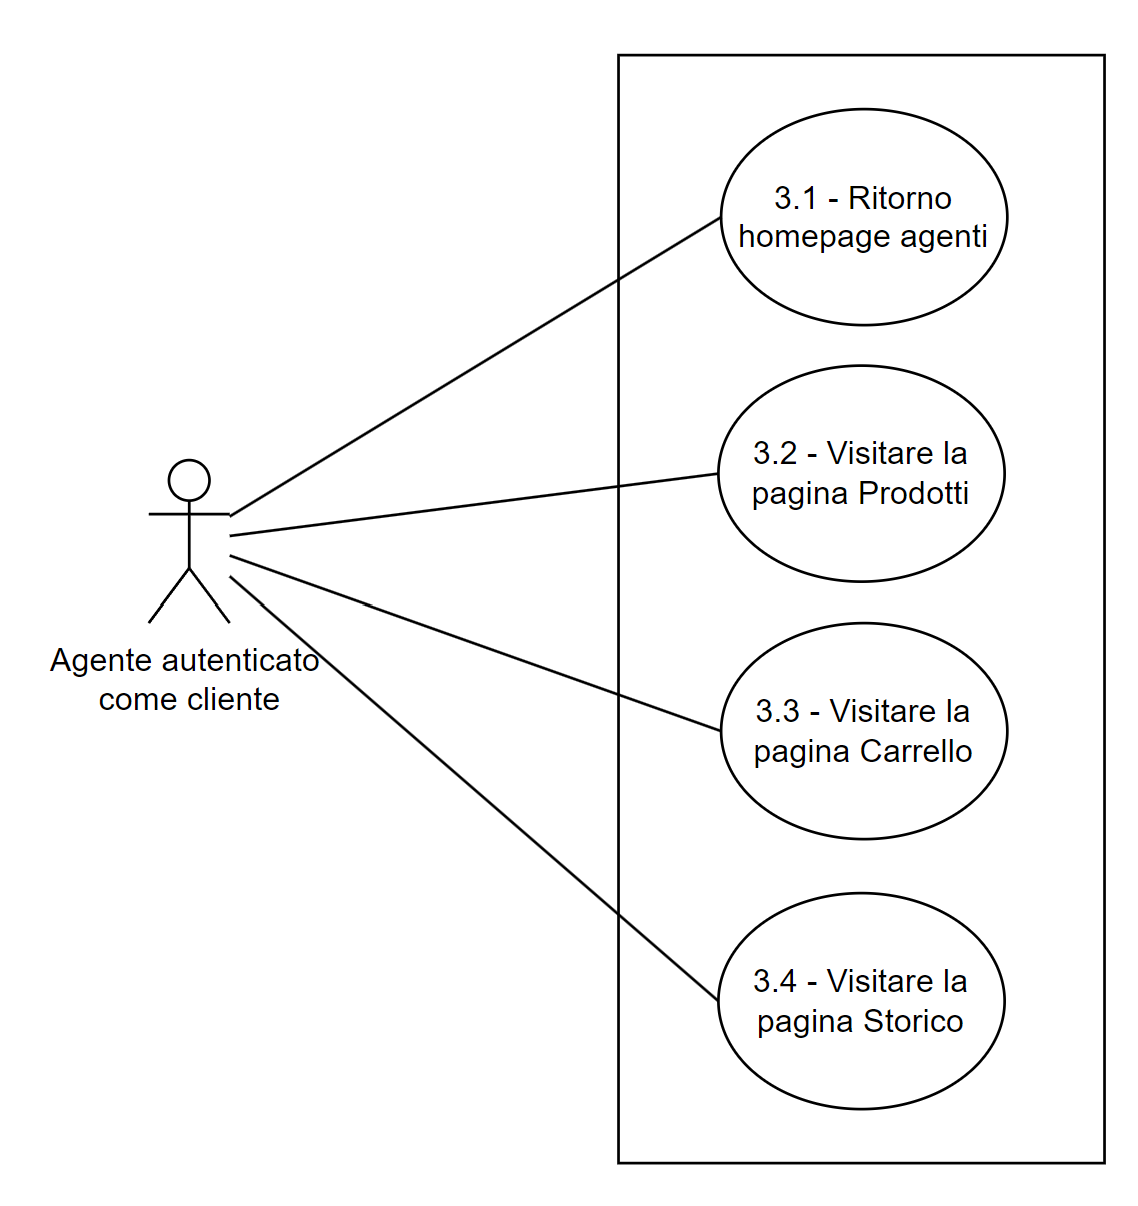
\includegraphics[width=0.75\columnwidth]{img/usecase/UC 3.png}
    \caption{\textit{Use Case} 3: Operazioni disponibili nella \textit{homepage} per agenti}
    \label{fig:uc_3}
\end{figure}

\begin{usecase}{ 3.1}{Ritorno \textit{homepage} agenti}
    \usecaseactors{Agente.}
    \usecasedesc{L'agente, cliccando nell'apposito menu il pulsante "\textit{Homepage} Agenti", ritorna alla 
                 \textit{homepage} agenti.}
    \usecasepre{L'agente ha selezionato un cliente dalla lista.}
    \usecasepost{L'agente si è spostato nella \textit{homepage} agenti.}
    \usecasescen{
        \begin{itemize}
            \item L'agente seleziona un cliente della lista;
            \item L'agente viene spostato nella \textit{homepage};
            \item L'agente può operare nell'\textit{app} come il cliente selezionato;
            \item L'agente preme il pulsante "\textit{Homepage} Agenti";
            \item L'agente ritorna alla \textit{homepage} agenti.
        \end{itemize}}
    \label{uc:uc_3.1}
\end{usecase}

\begin{usecase}{ 3.2}{Visitare la pagina Prodotti}
    \usecaseactors{Agente.}
    \usecasedesc{L'agente, cliccando nell'apposito menu il pulsante "Prodotti", può operare nella pagina 
                 Prodotti come il cliente selezionato.}
    \usecasepre{L'agente ha selezionato un cliente dalla lista.}
    \usecasepost{L'agente si è spostato nella pagina Prodotti.}
    \usecasescen{
        \begin{itemize}
            \item L'agente seleziona un cliente della lista;
            \item L'agente viene spostato nella \textit{homepage};
            \item L'agente preme il pulsante "Prodotti";
            \item L'agente viene spostato nella pagina Prodotti dove può operare come il cliente selezionato.
        \end{itemize}}
    \label{uc:uc_3.2}
\end{usecase}

\begin{usecase}{ 3.3}{Visitare la pagina Carrello}
    \usecaseactors{Agente.}
    \usecasedesc{L'agente, cliccando nell'apposito menu il pulsante "Carrello", può operare nella pagina 
                 Carrello come il cliente selezionato.}
    \usecasepre{L'agente ha selezionato un cliente dalla lista.}
    \usecasepost{L'agente si è spostato nella pagina Carrello.}
    \usecasescen{
        \begin{itemize}
            \item L'agente seleziona un cliente della lista;
            \item L'agente viene spostato nella \textit{homepage};
            \item L'agente preme il pulsante "Carrello";
            \item L'agente viene spostato nella pagina Carrello dove può operare come il cliente selezionato.
        \end{itemize}}
    \label{uc:uc_3.3}
\end{usecase}

\begin{usecase}{ 3.4}{Visitare la pagina Storico}
    \usecaseactors{Agente.}
    \usecasedesc{L'agente, cliccando nell'apposito menu il pulsante "Storico", può operare nella pagina 
                 Storico come il cliente selezionato.}
    \usecasepre{L'agente ha selezionato un cliente dalla lista.}
    \usecasepost{L'agente si è spostato nella pagina Storico.}
    \usecasescen{
        \begin{itemize}
            \item L'agente seleziona un cliente della lista;
            \item L'agente viene spostato nella \textit{homepage};
            \item L'agente preme il pulsante "Storico";
            \item L'agente viene spostato nella pagina Storico dove può operare come il cliente selezionato.
        \end{itemize}}
    \label{uc:uc_3.4}
\end{usecase}

\subsubsection{UC 4 - Cambio tema}
\begin{figure}[H]
    \vspace{2em}
    \centering
    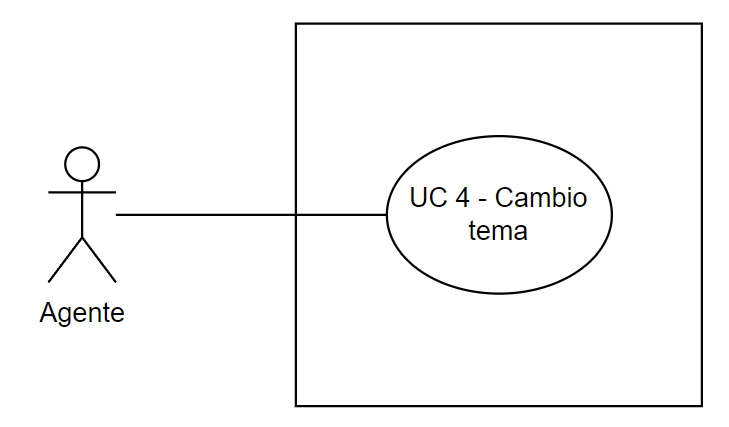
\includegraphics[width=0.75\columnwidth]{img/usecase/UC 4.png}
    \caption{\textit{Use Case} 4: Cambio tema}
    \label{fig:uc_4}
\end{figure}

\begin{usecase}{ 4}{Cambio tema}
    \usecaseactors{Agente.}
    \usecasedesc{L'agente cambia il tema dell'applicazione in chiaro o scuro.}
    \usecasepre{L'agente, dalla \textit{homepage} agenti, cliccando nell'apposito menu il pulsante "Impostazioni", si 
                sposta nella pagina Impostazioni.}
    \usecasepost{L'agente ha cambiato il tema dell'\textit{app}.}
    \usecasescen{
        \begin{itemize}
            \item L'agente si trova nella \textit{homepage} agenti;
            \item L'agente preme il pulsante "Impostazioni" dal menu;
            \item L'agente viene spostato nella pagina Impostazioni;
            \item L'agente cambia il tema dell'applicazione.
        \end{itemize}}
    \label{uc:uc_4}
\end{usecase}

\subsubsection{UC 5 - \textit{Logout}}
\begin{figure}[H]
    \vspace{2em}
    \centering
    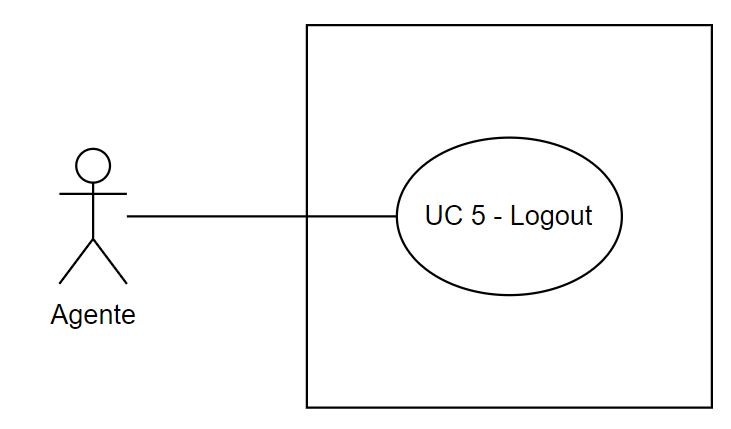
\includegraphics[width=0.75\columnwidth]{img/usecase/UC 5.png}
    \caption{\textit{Use Case} 5: \textit{Logout}}
    \label{fig:uc_5}
\end{figure}

\begin{usecase}{ 5}{\textit{Logout}}
    \usecaseactors{Agente.}
    \usecasedesc{L'agente effettua la procedura di \textit{logout}.}
    \usecasepre{L'agente, dalla \textit{homepage} agenti, cliccando nell'apposito menu il pulsante "Account", si 
                sposta nella pagina Account.}
    \usecasepost{L'agente ha effettuato il \textit{logout} e torna un utente non autenticato. 
                 L'agente viene spostato alla pagina di \textit{login}.}
    \usecasescen{
        \begin{itemize}
            \item L'agente si trova nella \textit{homepage} agenti;
            \item L'agente preme il pulsante "Account" dal menu;
            \item L'agente viene spostato nella pagina Account;
            \item L'agente effettua il \textit{logout};
            \item L'agente torna un utente non autenticato;
            \item L'agente viene spostato alla pagina di \textit{login}
        \end{itemize}}
    \label{uc:uc_5}
\end{usecase}
